% Pembelajaran mesin sudah banyak dipakai di berbagai bidang keilmuan. seperti penelitian yang dilakukan oleh Lawrence  pada tahun 2007
% dengan judul 
% untuk mendeteksi wajah \cite{lawrence1997face}
% Mulai dari Pemrosesan citra seperti yang di lakukan oleh   . Dalam papernya dia menggunakan \emph{neural network} dengan tipe \emph{Convolutional Neural Network} untuk mendeteksi wajah. 

% Van Gent et al (2007) \cite{van2007neural}, 
% dia menggunakan \emph{Neural Network} untuk menganalisa \emph{overtopping} gelombang pada struktur di wilayah pantai. 

% Yau et al (2012)\cite{YAO201230}, dalam papernya dia menggunakan model \emph{Boussinesq} 1 dimensi untuk memodelkan transformasi gelombang ketika melewati terumbu karang. Pada bab ini dijelaskan model \emph{runup} gelombang pada terumbu karang menggunakan Pembelajaran Mesin.
\subsection{Runup Gelombang}
Runup gelombang adalah jarak vertikal maksimum dari kenaikan gelombang pada pantai atau struktur di atas \emph{SWL} \cite{sorensen2005basic}. Dalam penelitian ini, data ovservasi ketinggian \emph{runup} gelombang diukur mulai ketinggian \emph{swl}, hingga maksimum ketinggian air di daratan. Penjelasan lebih lanjut tentang pengambilan data dijelaskan pada bagian \nameref{kondisiEksperimen}. Runup gelombang dapat diilustrasikan pada gambar \ref{fig:runup}.
\begin{figure}[h]
    \begin{center}
        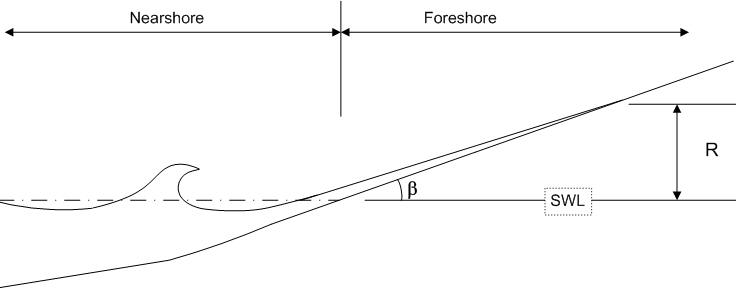
\includegraphics[scale=0.7]{./images/runup_gelombang.jpg}
    \end{center}
    \caption{Ilustrasi \emph{Runup} gelombang oleh Mike Swenson, Coastal Morphology, University of Wisconsin-Madison \cite{MikeSwenson:WaveRunup}.}
    \label{fig:runup}
\end{figure}
\FloatBarrier
Pada gambar.\ref{fig:runup} \emph{SWL (Sea Water Level)} adalah ketinggian air normal ketika tidak ada gelombang. Wilayah Pantai (\emph{Foreshore}) dimulai dari titik \emph{SWL} yang berpotongan dengan daratan. Wilayah lautan (\emph{Nearshore}) dimulai dari titik \emph{SWL} yang berpotongan dengan air. Ketika titik potong air dengan daratan berada di atas \emph{SWL}, maka kondisi tersebut dinamakan dengan \emph{runup}. Ketinggian \emph{runup} dinotasikan dengan $R$. Simbol $\upbeta$ melambangkan kemiringan bibir pantai.

\subsection{Pembelajaran Mesin}

Pembelajaran mesin adalah bidang studi yang memberikan kemampuan komputer untuk belajar, tanpa harus di program secara khusus \cite{arthur_l_samuel_1959}. Mesin dikatakan belajar dari pengalaman ($E$) terhadap tugas ($T$) dan ukuran kinerja ($P$), jika kinerja pada tugas ($T$), yang di ukur berdasarkan ($P$), berkembang berdasarkan pengalaman ($E$). Dalam TA ini, akan dibuat suatu program yang dapat belajar dari data gelombang hasil observasi ($T$). Lalu dievaluasi hasilnya dengan menggunakan $MSE$ ($P$), sehingga dapat di lihat seberapa besar galatnya. Lalu diperkecil galatnya dengan metode optimasi.

% \subsubsection{Supervised Learning}

% Sebelum data dimasukan ke dalam program, data tersebut diberikan label. Label tersebut bisa berupa \emph{input}, yakni $H$ (\emph{Significant Height} Gelombang), $T$ (\emph{Spectral Peak Periods}), dan $WL$ (\emph{Wave Length}). Dan label untuk \emph{output}. Karna pada TA kali ini, akan digunakan regresi linear. Maka tidak ada label untuk \emph{output}. Parameter \emph{input} yang berpasangan dengan \emph{output} tertentu, selanjutnya dinamakan contoh. Pembelajaran Mesin yang demikian dinamakan \emph{Supervised Learning}. \emph{Supervised Learning} Merupakan bagian dari pembelajaran mesin yang memetaan \emph{input} ke \emph{output} yang berdasar pada contoh pasangan \emph{input} dan \emph{output}\cite{AIPeterNorvig}. 

\subsubsection{Neural Network}

\emph{Neural network} pertama kali didefenisikan oleh McCulloch-Pitts pada tahun 1943 \cite{McCulloch1943}. \emph{Neural network} adalah model matematika atau model komputasi untuk memproses informasi berdasarkan pendekatan koneksionis ke komputasi, perilaku globalnya ditentukan oleh koneksi antara elemen pemrosesan dan parameter elemen\cite{gurney2014introduction}.
Arsitektur \emph{Neural network} terdiri dari \emph{Input neuron}, \emph{hidden layer} dan \emph{Output neuron}. Arsitektur \emph{Neural network} dapat dilihat pada gambar 
\ref{fig:neural_network_sederhana}

\begin{figure}[H]
    \centering
    \def\layersep{4cm}
    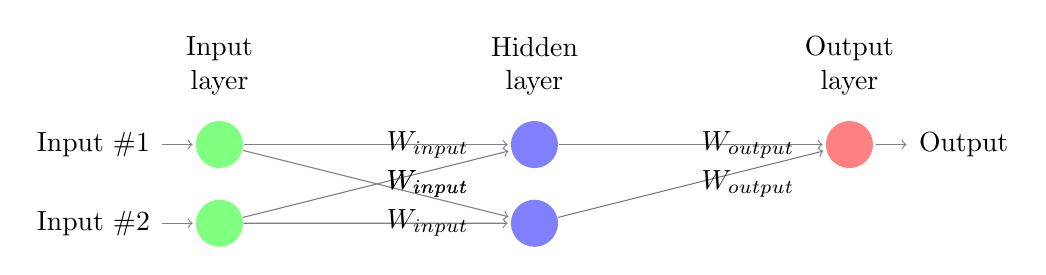
\begin{tikzpicture}[shorten >=1pt,->,draw=black!50, node distance=\layersep]
        \tikzstyle{every pin edge}=[<-,shorten <=1pt]
        \tikzstyle{neuron}=[circle,fill=black!25,minimum size=17pt,inner sep=0pt]
        \tikzstyle{input neuron}=[neuron, fill=green!50];
        \tikzstyle{output neuron}=[neuron, fill=red!50];
        \tikzstyle{hidden neuron}=[neuron, fill=blue!50];
        \tikzstyle{annot} = [text width=4em, text centered]

        % Draw the input layer nodes
        \foreach \name / \y in {1,...,2}
        % This is the same as writing \foreach \name / \y in {1/1,2/2,3/3,4/4}
            \node[input neuron, pin=left:Input \#\y] (I-\name) at (0,-\y) {};

        % Draw the hidden layer nodes
        \foreach \name / \y in {1,...,2}
            \path[yshift=0.0cm]{}
                node[hidden neuron] (H-\name) at (\layersep,-\y cm) {};

        % Draw the output layer node
        \node[output neuron,pin={[pin edge={->}]right:Output}, right of=H-1] (O) {};

        % Connect every node in the input layer with every node in the
        % hidden layer.
        \foreach \source in {1,...,2}
            \foreach \dest in {1,...,2}
                \path (I-\source) edge node[midway, right] {$W_{input}$} (H-\dest);

        % Connect every node in the hidden layer with the output layer
        \path (H-1) edge node[midway, right] {$W_{output}$} (O);
        \path (H-2) edge node[midway, right] {$W_{output}$} (O);

        % Annotate the layers
        \node[annot,above of=H-1, node distance=1cm] (hl) {Hidden layer};
        \node[annot,left of=hl] {Input layer};
        \node[annot,right of=hl] {Output layer};
        \label{neuralNetworkRepresentation}
    \end{tikzpicture}
    \caption{Model \emph{Neural Network} dengan 1 \emph{Hidden Layer}.}
    \label{fig:neural_network_sederhana}
\end{figure}

Pada umumnya persamaan \emph{Neural network} dapat dilihat pada pers.\ref{eq:regresi} dimana nilai z dapat dilihat pada pers.\ref{eq:mcullochNeuralNetwork}
\begin{equation}
    \label{eq:regresi}
    y = f(z)
\end{equation}

\begin{equation}
\label{eq:mcullochNeuralNetwork}
    z = \sum_{i=1}^N I_iW_i
\end{equation}

Dimana y adalah output, $I$ merupakan output dari neuron sebelumnya, $W_{i}$ adalah bobot atau \emph{Weight}, f(z) adalah nilai aktivasi dari hasil penjumlahan dari perkalian input dengan bobot. Fungsi aktivasi yang digunakan adalah fungsi aktivasi linear dan ReLU. 

\subsubsection{Fungsi Aktivasi}

Fungsi aktivasi digunakan untuk mengubah level aktivasi pada suatu neuron menjadi sebuah sinyal output \cite{KarlicOlgacPerformanceAnalysis}. Dalam penelitian ini fungsi aktivasi yang digunakan pada hidden layer adalah  fungsi aktivasi \emph{Rectified Linear Unit (RELU)}\cite{glorot2011deep}. Fungsi aktivasi \emph{RELU} didefinisikan dengan persamaan \ref{eq:aktivasi_relu}  dan fungsi aktivasi linear \cite{MLBishop}. pada pers.\ref{eq:aktivasi_linear}

\begin{equation} 
    \label{eq:aktivasi_relu}
ReLU (x)=\begin{cases} 0, & \mbox{if} x\le 0 \\ x, & \mbox{if} x > 0 \end{cases}
\end{equation}

\begin{equation}
    \label{eq:aktivasi_linear}
    y=x
\end{equation}

% RELU menjadi pilihan karna memiliki performa konvergensi yang lebih baik dibanding sigmoid \cite{Krizhevsky:2012:ICD:2999134.2999257}. 

\subsubsection{Estimasi Galat / \emph{Cost / Lost Function}}

Kalkulasi galat sangat penting untuk menentukan seberapa besar akurasi yang dimiliki model prediksi pada TA ini. Fungsi estimasi galat yang digunakan adalah \emph{Mean Square Error (MSE)}. Persamaan MSE didefinisikan dengan

\begin{equation}
    \operatorname{MSE}=\frac{1}{n}\sum_{i=1}^n(Y_i-\hat{Y_i})^2,
\end{equation}

dimana $Y$ adalah ketinggian gelombang hasil observasi, $\hat{Y}$ adalah ketinggian gelombang hasil prediksi, dan $n$ adalah jumlah data training.

% TODO:fix gambar instrumen eksperimen